\documentclass[a4paper,12pt]{article}

\usepackage{indentfirst}
\usepackage[utf8]{inputenc}
\usepackage{graphicx}
\usepackage{float}
\usepackage[portuguese]{algorithm2e}
\usepackage{amsmath}
\usepackage{listings}
\title{Chat assíncrono criptografado utilizando  sockets TCP em Java}
\author{Sila Geroges Agiru Judick Siebert\\UDESC
        \and Wagner Luis Sousa da Luz \\UDESC}
\date{\today}


\begin{document}

\maketitle

\begin{abstract}
\noindent Isto é um resumo do artigo.\\
Síntese (2 ou 3 parágrafos) com a ideia principal do artigo.
\end{abstract}


\section{Introdução}
\subsection{Objetivo}
Você deve implementar uma sala de bate-papo, com N conexões, criptografia nas mensagens e todos
os terminais devem exibir a mesma ordem as mensagens recebidas.
\subsubsection{Problema}
Considerações
a criptografia deve inverter valor dos bits da mensagem.
Devem utilizar uma conexão TCP/IP
não utilizar a classe bufferedreader e bufferedwriter
              
A figura \ref{fig1} representa uma sala de bate-papo.
\begin{figure}[H]
	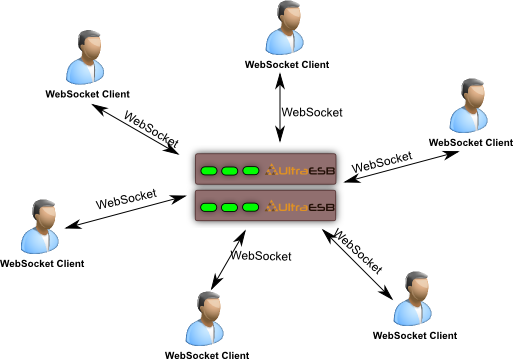
\includegraphics[scale=0.63]{img/454.png}    
	\caption{Sala de bate-papo}
	\label{fig1}     
\end{figure} 

\section{A sua Implementação}

A figura \ref{fig2} representa o diagrama de classe da nossa implementação.
\begin{figure}[H]
	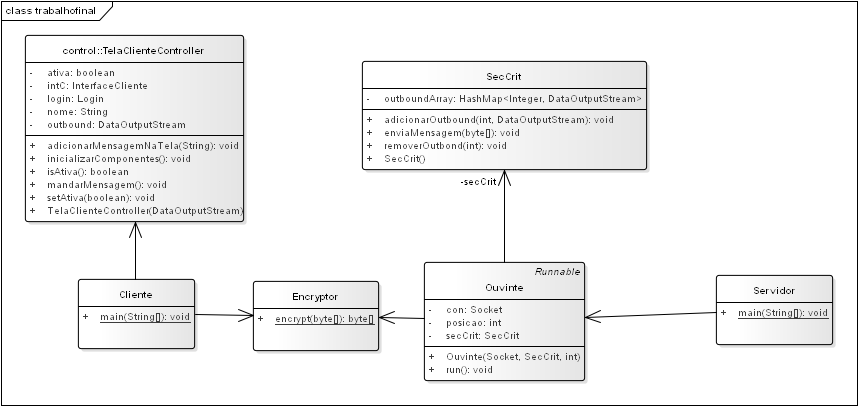
\includegraphics[scale=0.5]{img/class.png}    
	\caption{Class diagram}
	\centering
	\label{fig2}
\end{figure} 

\lstinputlisting[language=Java, firstline=8]{../../TrabalhoFinal/src/trabalhofinal/Servidor.java}


A figura \ref{fig3} representa o diagrama de atividade da classe servidor da nossa
implementação.
\begin{figure}[H]
	\centering
	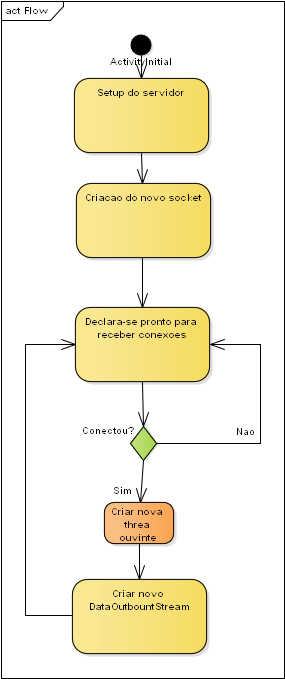
\includegraphics[scale=0.5]{img/serverflow.png}    
	\caption{Activity diagram do servidor}
	
	\label{fig3}
\end{figure}
\section{Avaliação}
A equação (\ref{for1})  apresenta uma integral de 0 a $\infty$.
\begin{align}
	\label{for1}	\int_0^\infty e^{-x^2} dx=\frac{\sqrt{\pi}}{2}
\end{align}


\section{Avaliação da implementação}

\section{Conclusão}
Síntese do que foi dito.\\
Lista dos resultados atingidos:
\begin{itemize}
\item resultado 1
\item resultado 2 e teste de bibliografia \cite{Bulfinch1998}
\end{itemize}
Conclusão final e Trabalho Futuro.

\bibliographystyle{plain}
\bibliography{n2library.bib}

\end{document}
